\chapter{Sincronizzazione}

Quando due o più thread vengono eseguiti in parallelo devono essere sincronizzati correttamente per evitare l'insorgenza di race condition.

\section{Race Condition}
Quando più processi accedono in concorrenza e modificano i dati condivisi l'esito finale dell'esecuzione è indeterminato. Dipende dall'ordine in cui le loro istruzioni vengono eseguite.
Questa situazione viene chiamata \textbf{race condition} e va gestita per evitare di ottenere risultati erronei.

\subsubsection*{Esempio}

\spacer
\begin{minipage}{0.45\textwidth}
    \begin{minted}{java}
// Thread 1
for (int i = 0; i < 5; i++) {
    x++;
}
\end{minted}
\end{minipage}
\hfill
\begin{minipage}{0.45\textwidth}
    \begin{minted}{java}
// Thread 2
for (int j = 0; j < 5; j++) {
    x--;
}
\end{minted}
\end{minipage}
\spacer

In questo caso, se i due thread vengono eseguiti concorre mente, il valore finale di $x$ non è noto, potrebbe variare tra $-5$ e $+5$.

\subsubsection*{Operazioni Atomiche}

Per risolvere il problema della \textit{race condition} è necessario svolgere le operazioni di lettura e modifica delle variabili condivise senza interruzioni. Queste operazioni sono definite \textbf{atomiche}.

\section{Regioni Critiche}
Definiamo \textbf{Regioni Critiche} di un processo quelle regioni dove si accede ai dati in comune. Ci si deve quindi assicurare che solo un processo per volta possa entrare nella sua sezione critica.

\spacer
È importante gestire correttamente la sincronizzazione dei processi, ogni processo deve richiedere il permesso di entrare nella sezione critica e deve attendere che questo permesso gli sia garantito.

\spacer
Il protocollo di cooperazione tra processi deve garantire:
\begin{sitemize}
    \item \textbf{Mutua Esclusione:} un solo processo nella sezione critica per volta
    \item \textbf{Progresso:} Quando uno o più processi richiedono di entrare nella sezione critica la decisione deve essere fatta solo da processi che stanno già eseguendo la loro sezione critica o che potrebbero eseguirla in futuro. Ricordando sempre che la decisione non può essere rimandata indefinitamente.
    \item \textbf{Attesa Limitata:} Per evitare la \textit{starvation} è necessario limitare il tempo massimo di attesa.
\end{sitemize}

\subsubsection*{Kernel}
Anche le strutture dati del kernel, comprese quelle incaricate di gestire le risorse condivise, sono a loro volta suscettibili a race condition.

\spacer
È possibile risolvere questo problema utilizzando un kernel senza diritto di prelazione, quindi con processi che non escono dalla modalità kernel finché essi non si bloccano o restituiscono volontariamente il controllo alla CPU.

Questa è la soluzione utilizzata da Windows XP e Windows 2000, ma è particolarmente inefficiente per i sistemi multiprocessore e real-time.
Linux supporta la prelazione a partire dalla versione 2.6

\section{Lock}
In generale qualsiasi soluzione al problema della sezione critica utilizza il \textbf{lock}. Per accedere ad una sezione critica il processo deve acquisire un lock, che restituisce poi all'uscita dalla sezione critica.

\begin{minted}{java}
{
    //acquisisce il lock
    sezione critica
    //restituisce il lock
    sezione non critica
}
\end{minted}

\subsubsection*{Supporto Hardware}
Molte architetture forniscono il supporto hardware per implementare efficacemente i lock, inoltre alcune forniscono anche direttamente delle istruzioni atomiche.

\subsubsection*{Supporto Sistema Operativo}
Dato che le implementazioni hardware sono spesso inaccessibili ai programmatori, il sistema operativo fornisce degli strumenti per risolvere il problema.

Il più semplice è il \textbf{lock mutex}, permette di proteggere le sezioni critiche aggiungendo \texttt{acquire()} prima del segmento e \texttt{release()} al termine
\begin{minted}{java}
acquire() {
    while(!available) {}; // busy wait
    available = false;
}

release() {
    available = true;
}
\end{minted}

\section{Semafori}
I semafori sono uno strumento più avanzato per gestire la cooperazione di più processi.

\spacer
Un semaforo a N valori è una variabile $s$ intera e non negativa sulla quale si può effettuare:
\begin{sitemize}
    \item \textbf{Wait:} decrementa $s$ di 1 se $s>0$, altrimenti sospende il processo. (Oppure \textit{Probeer te verlagen}, P)
    \item \textbf{Signal:} Risveglia uno dei processi in attesa, se nessuno sta attendendo incrementa $s$ di 1. (Oppure \textit{Verhogen} V)
\end{sitemize}

\begin{minted}{java}
wait(S) {
    while(S <= 0) {}; // busy wait
    S--;
}

signal(S) {
    S++;
}
\end{minted}


Definiamo \textbf{Semaforo Contatore} il semaforo a valori in un dominio non limitato. Utile nel controllo di un numero finito di risorse, il semaforo viene inizializzato al numero di risorse disponibili.
\textbf{Semaforo Binario} assume solamente i valori 0 e 1, simile al lock mutex.

\subsection{Implementazione}
L'utilizzo del busy waiting rappresenta un problema per un processo multiprogrammato perché l'attesa spreca cicli di CPU che potrebbero essere usati da un'altro processo.

\spacer
Per risolvere questo problema si può associare ad ogni semaforo una coda di processi in attesa, spesso implementata tramite una queue (First In First Out).


\begin{minted}{java}
struct semaphore {
    int value;
    struct process* list; //puntatore al primo elemento della struttura dati
};

wait(semaphore *S) { 
    S->value--;
    if (S->value < 0) {
        add this process to S->list;
        sleep();
    }
}

signal(semaphore *S) { 
    S->value++;
    if (S->value <= 0) {
        remove a process P from S->list; 
        wakeup(P);
    }
}
\end{minted}

In questo caso $valore$ può essere $<0$, in quelle situazioni $|valore|$ è il numero di processi in attesa.

\subsection{Problemi di Utilizzo}
I semafori possono dare luogo a situazioni inaspettate che devono essere gestite attentamente.

\subsubsection*{Deadlock}
Si possono trovare situazioni in cui uno o più processi attendono risorse che possono essere liberate solo da uno degli altri processi in attesa.

\begin{minipage}{0.45\textwidth}
    \begin{minted}{java}
wait(S);
wait(Q);
...
signal(S);
signal(Q);
\end{minted}
\end{minipage}
\hfill
\begin{minipage}{0.45\textwidth}
    \begin{minted}{java}
wait(Q);
wait(S);
...
signal(Q);
signal(S);
\end{minted}
\end{minipage}

Linux fornisce uno strumento, lockdep, per rilevare i deadlock all'acquisizione di un lock.

\subsubsection*{Starvation}
Gestendo incorrettamente la lista associata al semaforo, per esempio utilizzando una struttura dati LIFO, è possibile che un processo attenda all'infinito nella coda senza mai venir rimosso.

\begin{figure}[H]
    \centering
    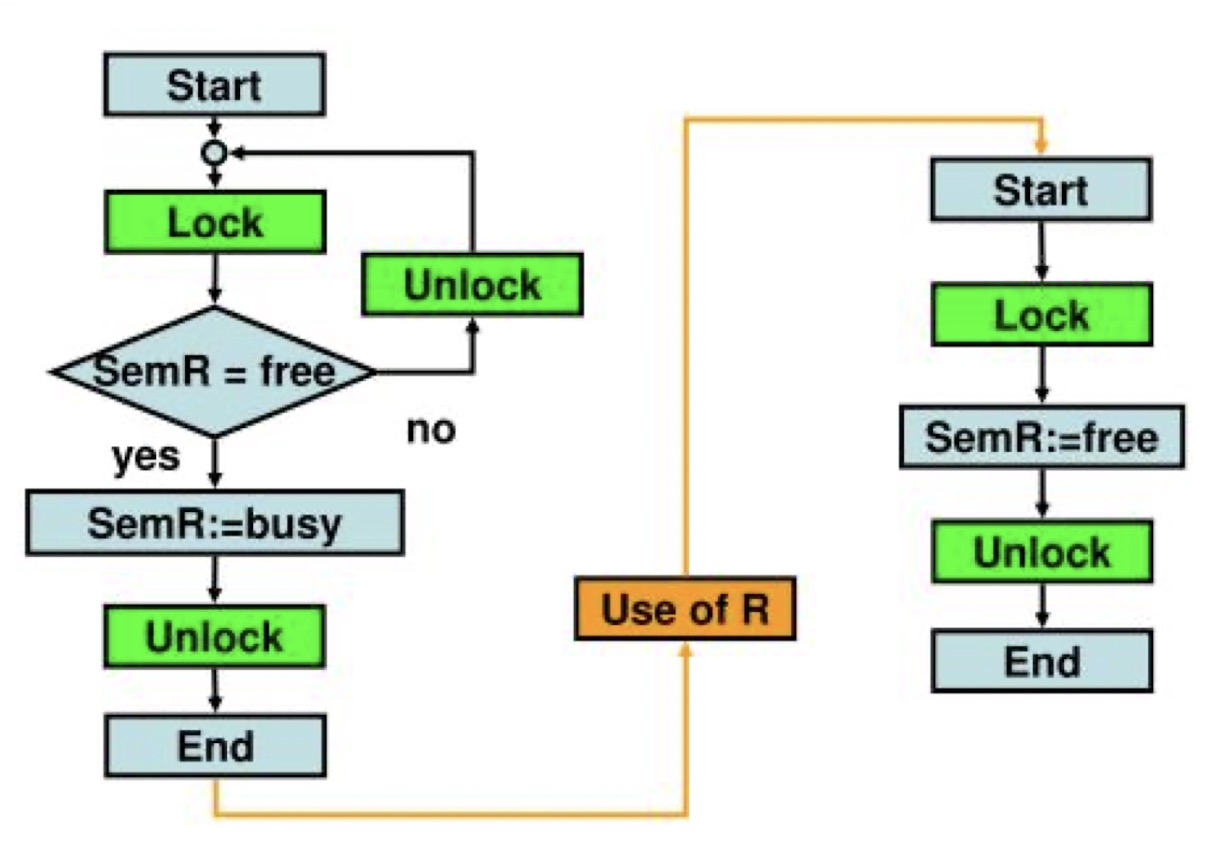
\includegraphics[width=0.5\linewidth]{assets/semaphore.jpg}
    \caption{Visualizzazione di un semaforo}
\end{figure}

\section{Monitor}
I semafori sono spesso utilizzare per sincronizzare l'utilizzo delle risorse, tuttavia il loro utilizzo incorretto può generare errori difficili da individuare.

\spacer
Un monitor è una struttura di più alto livello che contiene una serie di procedure e dei dati (condivisi tra i processi).
La caratteristica di un monitor è che al suo interno un solo processo per volta può essere attivo.

\begin{minted}{java}
monitor monitor_name {
    /* dichiarazioni delle variabili condivise */
    function P1 () {}
    function P2 () {}
    ...
    function PN () {}
}
\end{minted}

\subsection{Variabili Condition}
Le funzionalità appena descritte non sono sufficienti per modellare gran parte degli schemi di sincronizzazione.

Per questo vanno introdotte le variabili condition, da inserire tra le variabili condivise, sulle quali si possono effettuare solamente le operazioni di \texttt{wait()} e \texttt{signal()}.

Un processo può usare una variabile condition per attendere il verificarsi di una determinata condizione, uscendo dal monitor nell'attesa per lasciarlo libero ad altri processi.

\begin{figure}[H]
    \centering
    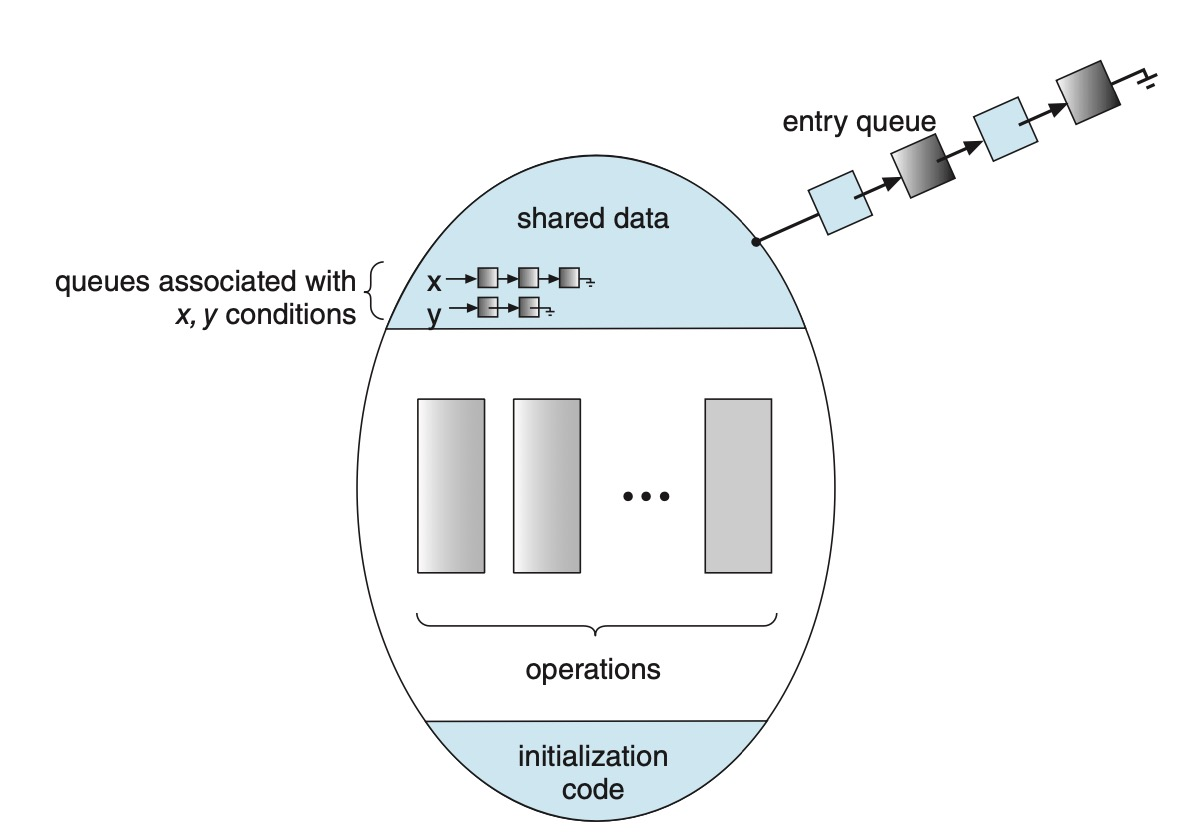
\includegraphics[width=0.6\linewidth]{assets/monitor.jpg}
    \caption{Monitor con variabili condition}
\end{figure}

\subsection{Gestione di signal}
Quando un processo $P$ invoca \texttt{signal()} su una risorsa che è attesa da un altro processo $Q$ si ottiene una situazione che può essere gestita in due modi:
\begin{sitemize}
    \item \textbf{Segnalare e attendere:} Il processo $P$, dopo la chiamata a \texttt{signal} esce dal monitor e lascia che $Q$ esegua la sua parte di codice.
    \item \textbf{Segnalare e procedere:} Il processo $P$ completa la sua esecuzione e poi $Q$ viene eseguito.
\end{sitemize}

\spacer
La seconda opzione, segnalare e procedere, sembra essere più ragionevole finché non si considera che la condizione che $P$ segnala potrebbe non essere più valida quando $Q$ arriva ad essere eseguito.

\section{Implementazione: Linux}
Prima della versione 2.6 (2004) Linux utilizzava un kernel senza diritto di prelazione. Per ottenere delle sezioni critiche venivano disabilitati momentaneamente gli interrupt.

\spacer
Ad oggi Linux fornisce diversi strumenti per la sincronizzazione:
\begin{itemize}
    \item \textbf{Lock Mutex:} Una variabile booleana che indica se il lock è disponibile, modificata tramite chiamate a sistema.
          \begin{minted}{cpp}
#include <pthread.h>
/* create and initialize the mutex lock */ 
pthread mutex t mutex;
pthread mutex init (&mutex, NULL);

pthread mutex lock (&mutex); /* acquire the mutex lock */ 
/* critical section */
pthread mutex unlock (&mutex); /* release the mutex lock */ 
    \end{minted}
    \item \textbf{Spinlock:} Un ciclo di busy waiting che verifica periodicamente se il lock è libero. È particolarmente inefficiente per i sistemi single core, in quanto altri processi non vengono eseguiti e quindi la risorsa attesa non viene sbloccata. Mentre può fornire alcuni vantaggi su sistemi multicore in quanto il processo non esce dall'esecuzione.
    \item \textbf{Semafori:} Ne esistono di due tipi, con e senza nome. I semafori con nome sono condivisi da tutti i processi imparentati, mentre quelli senza nome possono essere utilizzati solo nel contesto del processo.
          \begin{minted}{cpp}
#include <semaphore.h>
/* Create the semaphore and initialize it to 1 */
sem_t *sem;
sem = sem open ("SEM", O CREAT, 0666, 1);

sem_wait (sem); /* acquire the semaphore */
/* critical section */
sem-post (sem); /* release the semaphore */ 
            \end{minted}
    \item \textbf{Interi atomici:} Un tipo le cui operazioni sono tutte definite in modo atomico. Essi non risentono dell'overhead introdotto dai tradizionali meccanismi di lock.
          \begin{minted}{cpp}
atomic_t counter;
atomic_set (&counter, 5); /* counter = 5 */
atomic_add (10, &counter); /* counter = 15 */
atomic_sub (4, &counter); /* counter = 11 */
atomic_inc (&counter); /* counter = 12 */
int value = atomic_read (&counter); /* value = 12 */
    \end{minted}

    \item \textbf{Variabili condition:} Sono le variabili utilizzate per la realizzazione di monitor, forniscono un wait e un signal che gestiscono in autonomia un lock.

          Il wait acquisice periodicamente il lock, verifica la condition e poi libera il lock.

\end{itemize}

